\documentclass[11pt]{paper}

%%%%%%%%%%%%%%%%%%%%%%%%%%%%%%%%%%%%%%%%
% Basic packages
%%%%%%%%%%%%%%%%%%%%%%%%%%%%%%%%%%%%%%%%
\usepackage{amsmath,amsthm,amssymb}
\usepackage{mathtools}
\usepackage{etoolbox}
\usepackage{fancyhdr}
\usepackage{xcolor}
\usepackage{hyperref}
\usepackage{xspace}
\usepackage{comment}
\usepackage{url} % for url in bib entries
\usepackage{mathrsfs}


\theoremstyle{remark}
\newtheorem{theorem}{Theorem}
\newtheorem*{prop}{Proposition}
\newtheorem{problem}{Problem}
\newtheorem*{prob}{Problem}
\newtheorem*{solution}{{\bf Solution}}
\newtheorem*{hint}{{\it Hint}}

%%%%%%%%%%%%%%%%%%%%%%%%%%%%%%%%%%%%%%%%%%%%%%%%%%
%% Surround the problem and solution with 
%% \begin{ProbBox}  and   \end{ProbBox}
%% to prevent pagebreaks.
\newenvironment{ProbBox}{\noindent\begin{minipage}{\linewidth}}{\end{minipage}}

%%%%%%%%%%%%%%%%%%%%%%%%%%%%%%%%%%%%%%%%
% Acronyms
%%%%%%%%%%%%%%%%%%%%%%%%%%%%%%%%%%%%%%%%
\usepackage[acronym, shortcuts]{glossaries}

%% HERE IS HOW YOU DEFINE ACRONYMS:
\newacronym{FTA}{FTA}{Fundamental Theorem of Algebra}
\newacronym{CRT}{CRT}{Chinese Remainder Theorem}

% Make \ac robust.
\robustify{\ac}

\usepackage{enumerate}

\usepackage[
top    = 2cm,
bottom = 2cm,
left   = 3.00cm,
right  = 3.00cm]{geometry}

%%%%%%%%%%%%%%%%%%%%%%%%%%%%%%%%%%%%%%%%
% Fancy page style
%%%%%%%%%%%%%%%%%%%%%%%%%%%%%%%%%%%%%%%%
\pagestyle{fancy}
\newcommand{\metadata}[2]{
  \rhead{Midterm Exam}
  \chead{}
  \lhead{Math 700: Linear Algebra}
%  \lfoot{#1}\cfoot{#2}
  % \lfoot{}\cfoot{}
  % \rfoot{\thepage}
}
\renewcommand{\headrulewidth}{0.4pt}
\renewcommand{\footrulewidth}{0.4pt}

\newrobustcmd*{\vocab}[1]{\emph{#1}}
\newrobustcmd*{\latin}[1]{\textit{#1}}

%%%%%%%%%%%%%%%%%%%%%%%%%%%%%%%%%%%%%%%%
% Customize list enviroonments
%%%%%%%%%%%%%%%%%%%%%%%%%%%%%%%%%%%%%%%%
% package to customize three basic list environments: enumerate, itemize and description.
% \usepackage{enumitem}
% \setitemize{noitemsep, topsep=0pt, leftmargin=*}
% \setenumerate{noitemsep, topsep=0pt, leftmargin=*}
% \setdescription{noitemsep, topsep=0pt, leftmargin=*}

%%%%%%%%%%%%%%%%%%%%%%%%%%%%%%%%%%%%%%%%
%% Space between problems
\newrobustcmd*{\probskip}{\vskip1cm}

\usepackage{tikz}
\usetikzlibrary{matrix,arrows}
%% 
         \newcommand\alg[1]{\ensuremath{\mathbf{#1}}}
         \newcommand{\<}{\ensuremath{\langle}}
         \renewcommand{\>}{\ensuremath{\rangle}}
         \newcommand\fld[1]{\ensuremath{\mathbb{#1}}}
         \newcommand\GF{\ensuremath{\operatorname{GF}}}
         \newcommand\End{\ensuremath{\operatorname{End}}}
         \newcommand\Hom{\ensuremath{\operatorname{Hom}}}
         \newcommand\im{\ensuremath{\operatorname{im}}}

         \metadata{Math 700}{Midterm Exam -- 2014/03/07}
         \author{}
%%
%%    8. Update the title and date as appropriate.
         \title{Midterm Exam}
         \subtitle{Math 700: Spring 2014}
         \date{6 March 2014}



\begin{document}

\maketitle

\noindent {\bf INSTRUCTIONS} 
\begin{itemize}
\item 
Solve all of the problems below and then write up your solutions (neatly!),
giving complete proofs/justifications for all arguments.
Since this is a take home exam, I expect the presentation quality to be higher
quality than if this were an in-class exam.

\medskip

\item The questions are meant to test your understanding of basic  concepts, so you
should be more explicit than would if, say, you were writing an
article for a journal. In particular, it will help if you write down definitions
of any technical terms you use, even if these terms have already been mentioned
in the statement of the problem. In the first problem, for instance, you should
say what it means to be a projection, isomorphism, etc.  Of course, you must use your
best judgement about which definitions to state.  (You probably don't want to
provide definitions of the integers or real numbers, for example.)

\medskip

\item {\it Honor code.} You are expected to solve the exam problems on your own
  without outside help.  You may consult the lecture notes and textbook for this
  course only.  No other books or internet usage is allowed.\footnote{There is
    one exception to this rule, since I've asked you to look at a specific
    Wikipedia page when solving Problem~\ref{prob:sequences}.} 
  If you get stuck, please ask \emph{me} for
  help, in which case I might be willing to provide hints on our wiki page.

\item Finally, it will be helpful if you

\begin{enumerate}
\item 
state what you are trying to prove,
\item 
mention informally how you plan to prove it before giving the formal details, and
\item if you believe your proof is complete, use an end-of-proof symbol (like
  QED or \qedsymbol) to indicate this; on the other hand, if you believe your proof is
  incomplete, please say so.
\end{enumerate}
\end{itemize}

\noindent {\bf NOTATION}\\[4pt]
For the most part, we follow the notation used in the textbook.
Recall that if $V$ is a vector space over the field $F$ and if
$c\in F$, then $\sigma_c v = cv$ for all $v \in V$.
In particular, $\sigma_0$ and $\sigma_1$ denote the zero and identity maps,
respectively. 
\newpage

%%%%%%%%%%%%%%%%%%%%%%%%%%%%%%%%%%%%%%%%%%%%%%%%%%%%%%%%%%%%%%%%%%%%%%%%%%%%
\begin{problem} Let $V$ be a finite dimensional vector space over a field $F$.
Suppose $\alpha \in \End(V)$ is a projection with $X = \ker(\alpha)$ and $Y = \im(\alpha)$.
Define an isomorphism $\varphi: V \cong X \oplus Y$ (i.e., define the
appropriate map $\varphi$ and then prove that it is an isomorphism from 
$V$ onto $X \oplus Y$.
\end{problem}
\probskip




%%%%%%%%%%%%%%%%%%%%%%%%%%%%%%%%%%%%%%%%%%%%%%%%%%%%%%%%%%%%%%%%%%%%%%%%%%%%
\begin{problem}
\label{prob:sequences}
Suppose $V_0, V_1, V_2, \dots, V_n$ are vector spaces over the same field and
suppose that $f_k \in \Hom(V_k, V_{k+1})$, for each $0\leq k < n$.
We often use a diagram like the following to graphically depict such a sequence of maps:
\[
    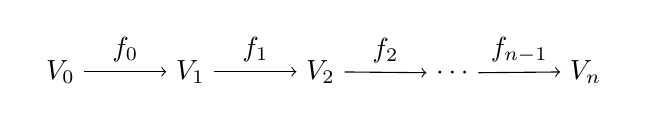
\begin{tikzpicture}
      \matrix (m) [matrix of math nodes, row sep=3em,column sep=3em]
      { V_0 & V_1 & V_2 & \cdots & V_n \\};
      \path[->] (m-1-1) edge node[above] {$f_0$}(m-1-2);
      \path[->] (m-1-2) edge node[above] {$f_1$}(m-1-3);
      \path[->] (m-1-3) edge node[above] {$f_2$}(m-1-4);
      \path[->] (m-1-4) edge node[above] {$f_{n-1}$}(m-1-5);
    \end{tikzpicture}
\]
    % \begin{tikzpicture}
    %   \matrix (m) [matrix of math nodes, row sep=3em,column sep=3em]
    %   { 0 & X & V & Y & 0 \\};
    %   \path[->] (m-1-1) edge node[above] {$\subset$}(m-1-2);
    %   \path[->] (m-1-2) edge node[above] {$f$}(m-1-3);
    %   \path[->] (m-1-3) edge node[above] {$g$}(m-1-4);
    %   \path[->] (m-1-4) edge node[above] {$\sigma_0$}(m-1-5);

    % \end{tikzpicture}
\noindent We call this an \emph{exact sequence} if $\im(f_k) =
\ker(f_{k+1})$ holds for all $0\leq k < n-1$.

\begin{enumerate}[(a)]
\item 
Suppose the following is an exact sequence:
\[
    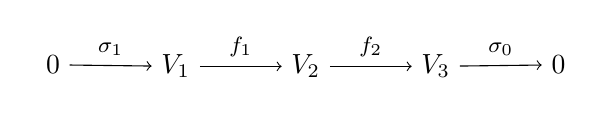
\begin{tikzpicture}
      \matrix (m) [matrix of math nodes, row sep=3em,column sep=3em]
      { 0 & V_1 & V_2 & V_3 & 0 \\};
      \path[->,font=\footnotesize] (m-1-1) edge node[above] {$\sigma_1$}(m-1-2);
      \path[->,font=\footnotesize] (m-1-2) edge node[above] {$f_1$}(m-1-3);
      \path[->,font=\footnotesize] (m-1-3) edge node[above] {$f_2$}(m-1-4);
      \path[->,font=\footnotesize] (m-1-4) edge node[above] {$\sigma_0$}(m-1-5);
    \end{tikzpicture}
\]
Then, what kind of homomorphism is $f_1$?  What about $f_2$?
\item Consider the following diagram:
\[
    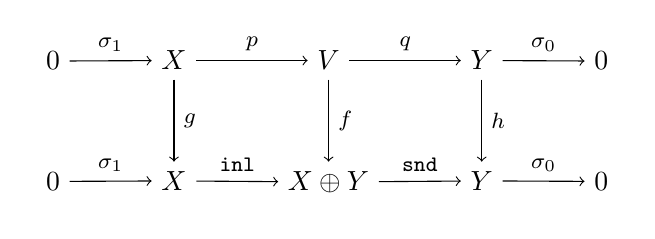
\begin{tikzpicture}
      \matrix (m) [matrix of math nodes, row sep=3em,column sep=3em]
      { 0 & X & V & Y & 0 \\
       0 & X & X\oplus Y & Y & 0 \\
      };
      \path[->,font=\footnotesize] (m-1-1) edge node[above] {$\sigma_1$}(m-1-2);
      \path[->,font=\footnotesize] (m-1-2) edge node[above] {$p$}(m-1-3);
      \path[->,font=\footnotesize] (m-1-3) edge node[above] {$q$}(m-1-4);
      \path[->,font=\footnotesize] (m-1-4) edge node[above] {$\sigma_0$}(m-1-5);

      \path[->,font=\footnotesize] (m-2-1) edge node[above] {$\sigma_1$}(m-2-2);
      \path[->,font=\footnotesize] (m-2-2) edge node[above] {{\tt inl}}(m-2-3);
      \path[->,font=\footnotesize] (m-2-3) edge node[above] {{\tt snd}}(m-2-4);
      \path[->,font=\footnotesize] (m-2-4) edge node[above] {$\sigma_0$}(m-2-5);

      \path[->,font=\footnotesize] (m-1-2) edge node[right] {$g$}(m-2-2);
      \path[->,font=\footnotesize] (m-1-3) edge node[right] {$f$}(m-2-3);
      \path[->,font=\footnotesize] (m-1-4) edge node[right] {$h$}(m-2-4);

    \end{tikzpicture}
\]
Here {\tt inl} denotes the left-inclusion map, 
\[
\mathtt{inl}: X \hookrightarrow X\oplus Y, \quad 
\mathtt{inl}: x\longmapsto x + 0,
\]
and {\tt snd} denotes the second-projection map,
\[
\mathtt{snd}: X \oplus Y \twoheadrightarrow Y, \quad 
\mathtt{snd}: x + y \longmapsto y.
\]
To complete this problem, first read the brief Wikipedia page on the \emph{Short Five Lemma}:
\url{http://en.wikipedia.org/wiki/Short_five_lemma}

Then, say how this lemma could be used in Problem 1 to prove that $\varphi$ is an
isomorphism.  In particular, give appropriate definitions for each of the maps
$p$, $q$, $f$, $g$,  and $h$ and say what else needs to be established about the
diagram in order to apply the lemma.\\
~[{\it Hint:} When defining the maps, choose from among the following: 
$\sigma_1$, $\alpha$, $\varphi$, $\sigma_1$.]
\end{enumerate}

\end{problem}
\probskip



%%%%%%%%%%%%%%%%%%%%%%%%%%%%%%%%%%%%%%%%%%%%%%%%%%%%%%%%%%%%%%%%%%%%%%%%%%%%
\begin{problem}

\end{problem}
\probskip



%%%%%%%%%%%%%%%%%%%%%%%%%%%%%%%%%%%%%%%%%%%%%%%%%%%%%%%%%%%%%%%%%%%%%%%%%%%%
\begin{problem}

\end{problem}
\probskip




\end{document}
